\chapter{Конструкторский раздел}
\label{cha:design}
\section{Общая архитектура приложения}
В состав приложения будет входить плагин для графического редактора, backend-сервер и frontend. Так же на бекенде будет размещена база данных
\begin{figure}[h!]
	\centering
	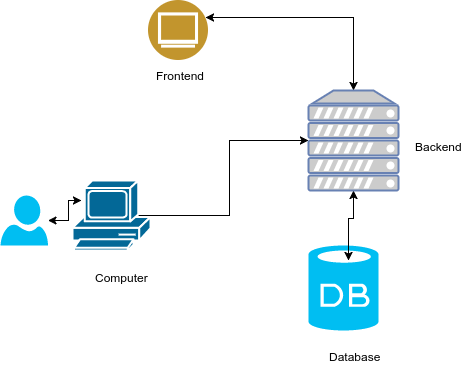
\includegraphics[width=0.6\textwidth]{img/diagram1.png}
	\caption{Общая архитектура приложения}
	\label{fig:spire01}
\end{figure}
\section{Клиентская часть}
\subsection{Библиотека KUserFeedback}
В качестве вспомогательной библиотеки для сбора стастики используется библиотека KUserFeedback компании KDAB. Эта библиотека включает в себя С++ Qt клиентскую часть, а так же сервер, написанный на PHP\cite{book3} Нам нет требуется их сервер и значительная часть функций, мы будем использовать только часть собирающую телеметрию. KUserFeedBack позволяет  собрать библиотеку по частям и линковать к нашему приложению только необхоимые модули. В программе используется модуль Core. Модуль Core содержит абстракный класс источника данных, от которого можно наследовать различные источники данных. Ниже представлено описание этого класса. В дальнейшем мы создадим классы, которые наследуются от этого абстрактого класса. В этих классах будут переопределеные все чисто виртуальноые функции. Ключевую роль будет играть переопределение функции \textit{data()} - именно это переопределение несет смысловую нагрузку класса.

 \begin{lstlisting}[language=c++,,escapeinside={(@}{@)},caption={struct file\_operations}] 

class KUSERFEEDBACKCORE_EXPORT AbstractDataSource
{
public:
virtual ~AbstractDataSource();

/* Возвращает имя ресурса
*  Этот метод используется только на сервере
*  и не должен показыватся пользователю
*/
QString name() const;

//Возвращает человеко-читаемое описание ресурса.
virtual QString description() const = 0;

//Возвращает данные, собранные ресурсом
virtual QVariant data() = 0;

// Загружает постоянное состояние для этого источника данных.
virtual void load(QSettings *settings);

//Сохраняет постоянное состояние для этого источника данных.    
virtual void store(QSettings *settings);

// Сбрасывает состояние источника данных
virtual void reset(QSettings *settings);

// Возвращает режим сбора данных
Provider::TelemetryMode telemetryMode() const;

//Изменяет режим сбора данных
void setTelemetryMode(Provider::TelemetryMode mode);

protected:
// Создает новый источник данных
explicit AbstractDataSource(const QString &name, Provider::TelemetryMode mode = Provider::DetailedUsageStatistics, AbstractDataSourcePrivate *dd = nullptr);

//Изменяет имя источника данных
void setName(const QString &name);

class AbstractDataSourcePrivate* const d_ptr;
private:
Q_DECLARE_PRIVATE(AbstractDataSource)
Q_DISABLE_COPY(AbstractDataSource)
};
}

 \end{lstlisting}

\subsection{Собираемые данные}
Основые собираемые данные приведены в таблице \ref{tab:collectdata}:
\begin{table}[h]
	\caption{\label{tab:collectdata}Описание собираемых данных}
	\begin{center}
		\begin{tabular}{|l|l|l|}
			\hline
			Информация о & Источник данных & Данные \\
			\hline \hline
			Инструменты & KisTool::activate, KisTool:deactivate & 
			CountUse float64 
			 \tabularnewline & & Time     float64 
			 \tabularnewline & & ToolName string \\
		
			\hline
			Действия & 
			KisMainWindows actioncollection()
			 & 
			CountUse float64 
			\tabularnewline & & TimeUse      float64 
			\tabularnewline & & ActionName string \\
			
			\hline
			Cвойства изображений & 
			KisDocument::saveFile()
			& 
			ColorProfile string 
			\tabularnewline & &  ColorSpace   string 
			\tabularnewline & & Height       float64 
			\tabularnewline & & Width      float64
			\tabularnewline & & Size      float64 
			\tabularnewline & & NumLayers      float64  \\

			\hline
		Информация  &
			KisDocument::saveFile()	& 
			AppVersion string 
			\tabularnewline о компьютере & &  CompilerVersion   string 
			\tabularnewline & & CompilerType      string 
			\tabularnewline & & CpuArchitecture      string
			\tabularnewline & & CpuCount     float64 
			\tabularnewline & & CpuFamily      float64  
			\tabularnewline & & CpuIsIntel    bool 
			\tabularnewline & & CpuModel      float64  
			\tabularnewline & & LocaleLanguage      string
			\tabularnewline & & OpenGlGlslVersion     string
			\tabularnewline & & OpenGlRenderer     string   
			\tabularnewline & & OpenGlVendor    string 
			\tabularnewline & & PlatformOs    string 
			\tabularnewline & & PlatformVersion    string 
			\tabularnewline & & QtVersion    string    
			\tabularnewline & & ScreenDpi    string 
			\tabularnewline & & ScreenHeight    string
			\tabularnewline & & ScrennWidth    string      \\            
				\hline
				Ассерты &
				kis\_assert\_common()	& 
				AssertFile string
				\tabularnewline & &  AssertLine float64
			 \tabularnewline & & 	AssertText string
			 \tabularnewline & & 	Count float64
			 \tabularnewline & & 	IsFatal bool \\
			\hline
		\end{tabular}
	\end{center}
	\end{table}
\subsection{Плагин для графического редактора}
Был разработан плагин для графического редактора Krita, который позволяет собирать телеметрию с пользователей. Телеметрия отправляется через определенные интервалы времени на удаленный сервер. Записи о действиях и инструментах отправляются каждые n минут. Информация о компьютере отправляется 1 раз при установке Krita. После этого в файл настроек записывается информация о том, что больше информацию о компьютере отправлять не стоит. Это позволяет избежать "замусоривания" отправляемой информации за счёт отсуствия дублирования. Информация об ассертах отправляется по мере необходимости. Если программа находится debug-режиме, программа аварийно завершает свою работу после любого ассерта. После того как аварийный ассерт сработал, он записывается в файл конфига Krita. При следующей запуске программы, он будет прочитан оттуда и отправлен на удаленный сервер при старте программы. Если программа собрана в release-версии, то при ассерте, не приводящем к аварийному завершению программы, информация об ассерте в рантайме программы отправляется на удаленный сервер.
Собираемые метрики агрегруются на стороне клиента в http-запрос. Тело запроса представляет собою JSON, пример этого JSON приведен ниже(форматирование нарушено в целях наглядности).
\begin{lstlisting}[language=c++,,escapeinside={(@}{@)},caption={Тело http-запроса}] 
{
"asserts": []
}

{
"Tools": [
{
"countUse": 1,
"timeUseMSeconds": 4581,
"toolName": "/Activate/KritaShape/KisToolLine"
},
{
"countUse": 4,
"timeUseMSeconds": 446,
"toolName": "/Use/KritaShape/KisToolBrush"
},
{
"countUse": 3,
"timeUseMSeconds": 417,
"toolName": "/Use/KritaShape/KisToolLine"
}]
}

{
"actions": [
{
"actionName": "file_save_as",
"countUse": 1,
"sources": "smth"
},
{
"actionName": "send_info",
"countUse": 2,
"sources": "smth"}]
}

{
"Images": [
{
"colorProfile": "RGB/Alpha",
"colorSpace": "sRGB-elle-V2-srgbtrc.icc",
"height": 1200,
"numLayers": 3,
"size": 0,
"width": 1600}]
}

{
"compiler": {
"type": "GCC",
"version": "5.4"
},
"cpu": {
"architecture": "x86_64",
"count": 4,
"family": 6,
"isIntel": true,
"model": 60
},
"general": {
"appLanguage": "ru",
"appVersion": "4.0.0-pre-alpha",
"systemLanguage": "en_US"
},
"opengl": {
"glslVersion": "1.30",
"renderer": "Haswell Mobile ",
"type": "GL",
"vendor": "Intel",
"vendorVersion": "Mesa 17.0.7",
"version": "3.0"
},
"platform": {
"os": "linux",
"version": "ubuntu-16.04"
},
"qtVersion": {
"value": "5.9.1"
},
"screens": [
{
"dpi": 101,
"height": 768,
"width": 1366}]
}
\end{lstlisting}
\subsection{Динамическое изменение данных}
Инструменты и действия(actions) могут меняться достаточно часто в процессе разработки графическего редактора. Поэтому неразумно задавать статически эти метрики в коде. В коде бекенд-сервера реализована поддержка добавления новых элементов. Раз в сутки просыпается новая горутина(легковесный тред), которая пробегается по базе данных и ищет новые инструменты и действия. После этого она записывает их в текстовый файл.  Подобное разумно применять не только для инструментов и действий, но и для любых часто изменяющихся данных. Поэтому подобная система реализована так же  для версий приложения. В будущем возможно расширения этой системы.
\subsection{Агрегация данных}
Было бы неразумно обращаться каждый раз к базе данных при запросе с фронтенда. Поэтому все данные предварительно кэшируются. Раз в n минут запускаются горутины, которые осуществляют запросы к базе данных и записывают полученные результаты в соответствующие структруры.
\begin{lstlisting}[language=c++,,escapeinside={(@}{@)},caption={Агрегация инструментов}] 
func AgregateTools() {
	file, err := os.Open("list_tools.txt")
	serv.CheckErr(err)
	defer file.Close()
	
	var ToolUse md.ToolsCollected
	var ToolActivate md.ToolsCollected
	var ToolsUse []md.ToolsCollected
	var ToolsActivate []md.ToolsCollected
	
	scanner := bufio.NewScanner(file)
	for scanner.Scan() {
		ToolUse.Name = scanner.Text()
		ToolUse.CountUse, ToolUse.Time = countToolsUse("/Use/" + ToolUse.Name)
		ToolsUse = append(ToolsUse, ToolUse)
		
		ToolActivate.Name = ToolUse.Name
		ToolActivate.CountUse, ToolActivate.Time = countToolsUse("/Activate/" + ToolActivate.Name)
		ToolsActivate = append(ToolsActivate, ToolActivate)
	}
	agregatedTools.ToolsActivate = ToolsActivate
	agregatedTools.ToolsUse = ToolsUse
	err = scanner.Err()
	serv.CheckErr(err)	
}
\end{lstlisting}
Эта функция требует пояснений. Во второй строчке открывается файл с предварительно сгенерированным списком инструментом. В цикле, который начинается со строчки 22, последовательно считываем названия инструментов из списка. После этого  обращаемся к базе данных и считаем сколько раз инструмент использовался и сколько в среднем заняло время этого использования. Начиная со строчки 27 считаем аналогично для активации/деактивации инструмента. Внутри функции countToolUse скрыто обращение к базе данных. Пример этого обращения приведен ниже. Первый запрос считает количество использований, второй считает среднее время использования. Запрос осуществляется при помощи библиотеки mgo - неофициальной обертки для MongoDB для языка Golang\cite{book1}
\begin{lstlisting}[language=c++,,escapeinside={(@}{@)},caption={Агрегация инструментов}] 
pipe := c.Pipe([]bson.M{{"$unwind": "$tools"}, {"$match": bson.M{"tools.toolname": name}}, {"$group": bson.M{"_id": "$tools.toolname", "total_count": bson.M{"$sum": "$tools.countuse"}}}})
pipe2 := c.Pipe([]bson.M{{"$unwind": "$tools"}, {"$match": bson.M{"tools.toolname": name}}, {"$group": bson.M{"_id": "$tools.toolname", "total_count": bson.M{"$avg": "$tools.time"}}}})
\end{lstlisting}
\section{Кэширование данных на фронтенде}
Очевидно, что неразумно каждый раз обращаться к бекенду за новыми данными. Поэтому данные на фронтенде тоже кэшируются в структуры, аналогичные структурам на бекенде.
Кэшировать данные на фронтенде и на бекенде может показаться излишним, однако, это помогает значительно увеличить скорость работы приложения, снизить нагрузку на сервер, позволить в дальнейшем легко масштабировать систему.
%%% Local Variables:

%%% mode: latex
%%% TeX-master: "rpz"
%%% End:
%--количество цветов
%||количество пикселей